\section{Path Heuristic with Imitation Learning}
\label{sec:approach}

%\jure{Notice notation here is using $v_s$, $v_g$, where s is start and t is target. This is not consistent with introduction. Let's fix intro to use the same terminology.}

\xhdr{Training objective} With the aim of minimizing $|\text{CLOSE}|$ after search, our goal is to train a parameterized heuristic function $h_{\theta} : \Psi \times \VS \times \VS \longrightarrow \mathbb{R}$ to predict ground-truth node distances $h^{*}$ and use $h_\theta$ within a greedy best-first policy $\pi_\theta$ at test time.  More specifically, we assume access to a distribution over graphs $P_{\mathcal{G}}$, a start-goal node distribution $P_{v_{sg}}(\cdot \: | \: \mathcal{G})$, and a time horizon $T$. Moreover, we assume a joint state-history distribution $s, \psi \sim P_s(\cdot \: | \: \mathcal{G}, t, \pi_{\theta}, v_s, v_g)$, where $P_s$ represents the probability our search being in state $s$, at time $0 \leq t \leq T$ on graph $\mathcal{G}$ with pathfinding problem $(v_s, v_g)$, with a greedy best-first search policy $\pi_{\theta}$ using heuristic $h_{\theta}$. Hence, our goal can be summarized as minimizing the following objective:

\begin{equation}
    \label{eq:obj}
    \mathcal{L}(\theta) = \mathop{\EX}_{\substack{\mathcal{G} \sim P_{\mathcal{G}}, \\ (v_s, v_g) \sim P_{v_{sg}} \\ t \sim \mathcal{U}(0, ..., T), \\ s, \psi \sim P_s}}\big[\frac{1}{|\text{OPEN}|}\sum_{v \in \text{OPEN}} (h^{*}(s, v, v_g) - h_{\theta}(\psi, v, v_g))^{2} \big]
\end{equation}

Before we describe the algorithm that can be used to minimize $\mathcal{L}$, we rewrite $h_{\theta}$ to include a memory digest component ($z_t$), which represents an embedding of $\psi$ at time step $t$. Hence, $h_\theta$ becomes $h_{\theta} : \mathbb{R}^{d} \times \mathcal{O} \times \VS \times \VS \longrightarrow \mathbb{R}$, where $d$ is the dimensionality of our memory's embedding space. As opposed to previous methods \cite{bhardwaj2017learning}, $z_{t}$ allows us to \textit{automatically extract} relevant features for heuristic computations and concurrently \textit{reduce the computational complexity} of the heuristic function. Further, as shown in \cite{bhardwaj2017learning}, if we would use $h_{\theta}$ to evaluate all actions in a state (i.e., recalculate the heuristic values of all nodes in $\text{OPEN}$), we would need a squared reduction in the number of expanded nodes compared with BFS for \phil to bring performance benefits over BFS, which however may not be possible on all datasets. Hence, we constrain the heuristic only to evaluate new $\text{OPEN}$ nodes which we obtain after moving a node to $\text{CLOSE}$, calling the set of new fringe nodes $\VS_{new}$ after each expansion. In practice, the policy $\pi_{\theta}$  yields an algorithm equivalent to greedy best-first search, with the heuristic function replaced by $h_{\theta}$.

%\jure{This is the first time we define policy $\pi$ and it is unclear that it actually refers to our work PHIL}  \update{Should be clearer now: $\pi_{\theta}$ mentioned at the beginning of approach and in background}

\subsection{Learning algorithm \& architecture}
\label{sec:ila}

\begin{algorithm}[t]
	\caption{\phil --- Sequential Heuristic Training}\label{alg:il_alg}
	Obtain hyperparameters $T$, $\beta_{0}$, $N$, $m$, $t_\tau$;\\
	Initialize $\mathcal{D} \leftarrow \emptyset$, $h_{\theta_{1}}$; \\ \label{lst:line:}
	\For{$i = 1, \ldots, N$}
	{   Sample $\mathcal{G} \sim P_{\mathcal{G}}$; \\
	    Sample $v_s, v_g \sim P_{v_{sg}}$; \\
	    Set $\beta \leftarrow \beta_0^{i}$; \\
        Set mixture policy $\pi_{mix} \leftarrow (1 - \beta) * \pi_{\theta_{i}} + \beta  * \pi^{*}$; \\
	    Collect $m$ trajectories $\tau_{ij}$ as follows; \\
		\For{$j = 1,\ldots,m$}
		{   
			Sample $t \sim \mathcal{U}(0, ..., T - t_{\tau})$;\\
			Roll-in $t$ time steps of $\pi_{\theta_{i}}$ to obtain $z_t$ and new state $s_t = (\text{CLOSE}^{0}, \text{OPEN}^{0}, \text{REST}^{0})$; \\
			Roll-out trajectory $\tau_{ij}$ as follows;\\
			\For{$k = 1,\ldots, t_{\tau}$}
		    {   
    			Update $s_{t + k - 1}$ using $\pi_{mix}$ to get new state $s_{t+k}$ and new fringe state $\text{OPEN}^{k}$; \\
    			Obtain new fringe nodes $\VS_{new} = \text{OPEN}^{k} \setminus \text{OPEN}^{k-1}$; \\
    			Update trajectory $\tau_{ij} \leftarrow \tau_{ij} \cup \{(\VS_{new}, h^{*}(s_{t+k}, \VS_{new}, v_g))\}$; \\
	        }
		    Update dataset $\mathcal{D} \leftarrow \mathcal{D} \cup \{(\tau_{ij}, z_t)\}$ or $\mathcal{D} \cup \{(\tau_{ij}, 0)\}$; \\	
	    }
	    Train $h_{\theta_{i}}$ using TBTT on each $\tau \in \mathcal{D}$ to get $h_{\theta_{i+1}}$;\\  
	}
	\Return{best performing $h_{\theta_{i}}$ on validation};
\end{algorithm}


% Describe algo
\xhdr{Imitation learning algorithm} In Algorithm \ref{alg:il_alg}, we present the pseudo-code of the IL algorithm used to train our heuristic models (Figure \ref{fig:il-proc}). The high-level idea of our algorithm is that we aggregate trajectories of search traces (i.e., sequences of new fringe nodes) and use truncated backpropagation through time to optimize $h_{\theta}$ after each data-collection step. In particular, after sampling a graph $\mathcal{G}$ and a search problem  $v_s, v_g$, we use our greedy learned policy $\pi_\theta$ induced by $h_\theta$ to roll-in for $t \sim \mathcal{U}(0, \dots, T - t_{\tau})$ expansions, where $T$ is the episode time horizon, and $t_\tau$ is the roll-out length. From our roll-in, we obtain a new state $s = (\text{CLOSE}^{0}, \text{OPEN}^{0}, \text{REST}^{0})$, and an initial memory state $z_t$. After our roll-in, we roll-out for $t_{\tau}$ steps using our mixture policy $\pi_{mix}$, which is obtained by probabilistically blending $\pi_\theta$ and the greedy best-first policy induced by the oracle heuristic $\pi^{*}$. In a roll-out, we collect sequences of new fringe nodes, together with their ground-truth distances to the goal $v_g$, given by $h^{*}$.  Once the roll-out is complete, we append the obtained trajectory and the initial state for the following optimization using backpropagation through time. Further analysis on the trade-offs between using rolled-in states $z_t$ or zeroed-out states for training can be found in the supplementary material.

Note that we could also use supervised learning-based approaches to sample a fixed dataset of ($v_s$, $v_g$, $h^{*}(s, v_s, v_g)$) 3-tuples and train a model to predict node distances conditioned on their features. However, our experiments in Section \ref{sec:experiments} demonstrate that ignoring the non-i.i.d. nature of heuristic search negatively impacts model performance, with supervised learning-based methods performing up to $40 \times$ worse.


%\jure{As one is reading this, the question besomese, why not just sample some paths, and learn a MLP or GNN in the IID setting to predict the shortest path distance from current node to goal. It would be good to have a quick paragraph here discussing why this is not a good idea and a forward pointer to experiments/ablations which show that imitation learning gives x\% improvement over IID learning.} \update{Wrote a short paragraph about this.}

\begin{figure}[!htpb]
    \centering
    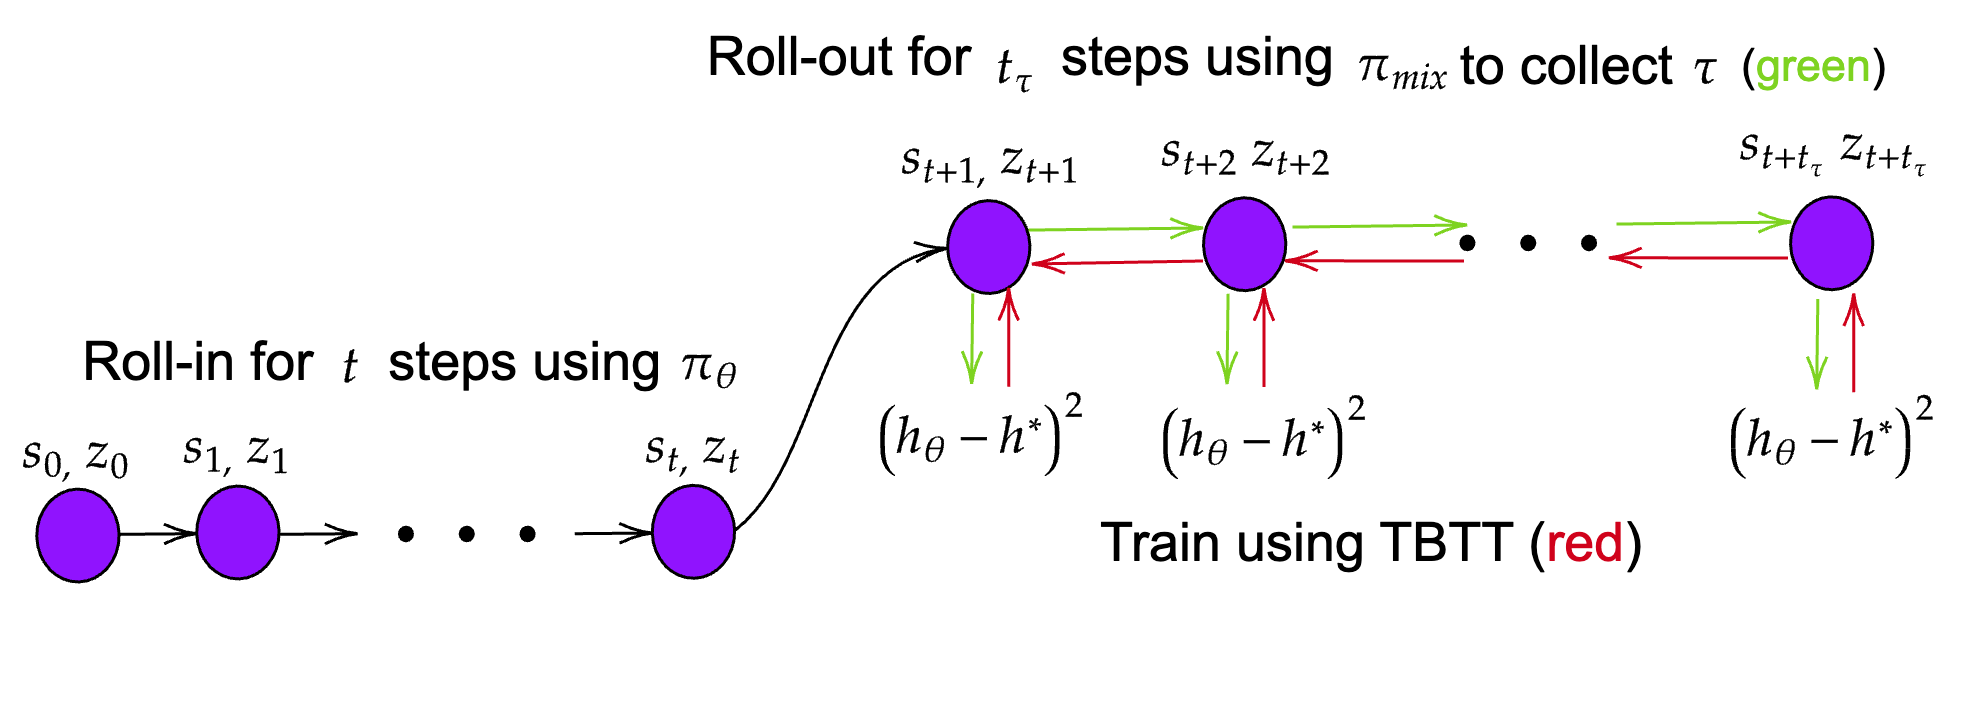
\includegraphics[width=0.9\textwidth]{figures/method_fig.png}
    \caption{This figure demonstrates the core idea behind our IL algorithm. We present the roll-in phase on the left-hand side, where our policy is rolled in for $t$ steps to obtain state $s_t$ and embedding $z_t$. On the right-hand side, we show the trajectory collection and training steps, where we aggregate the trajectory for downstream training (green) and use truncated backpropagation through time on the collected dataset (red).
    }
    \label{fig:il-proc}
    
\end{figure}

\begin{wrapfigure}[12]{R}{0.55\textwidth}
    \begin{algorithm}[H]
    	\caption{Heuristic func. ($h_\theta$) forward pass}\label{alg:htheta_alg}
    	 Obtain $x_i, x_j (j \in \mathcal{N}_i), e_{ij}, x_g$ $z_t$;\\
    	 $x_i \leftarrow f(x_i, x_g, D_{EUC}(x_i, x_g), D_{COS}(x_i, x_g)$);\\
     	 $x_j \leftarrow f(x_j, x_g, D_{EUC}(x_j, x_g), D_{COS}(x_j, x_g)$); \\
    
    	 $g_i \leftarrow \phi(x_i, \mathop{\oplus_{j \in \mathcal{N}_i}} \gamma(x_i, x_j, e_{ij}))$;\\
         $g^{\prime}_i, z_{i, t+1} \leftarrow \textsc{GRU}(g_i, z_t)$;\\
    	 $z_{t+1} \leftarrow \overline{z_{i, t+1}}$;\\ 
    	 $\hat{h}_i \leftarrow \textsc{MLP}(g^{\prime}_i, x_g);$\\
    	\Return{$\hat{h}_i ,z_{t+1}$};\\
    \end{algorithm}
\end{wrapfigure}


\textbf{Recurrent GNN architecture.} In each forward pass, $h_{\theta}$ obtains a set of new fringe nodes $\VS_{new}$, the goal node $v_g$, and the memory $z_t$ at time step $t$. We represent each node in $\VS_{new}$ using its features $x_{i} \in \mathbb{R}^{D_v}$, and likewise the goal node $v_g$ using its features $x_{g} \in \mathbb{R}^{D_v}$. Further, for each $i \in \VS_{new}$, we uniformly sample an $n \in \mathbb{N}_{\geq 0}$ bounded set of nodes present in the 1-hop neighborhood of $i$, calling this set $\mathcal{N}_i$, with $|\mathcal{N}_i| \leq n$. This sampling step produces a set of neighboring node features, where each $j \in \mathcal{N}_i$ has features $x_{j} \in \mathbb{R}^{D_v}$, and corresponding edge features $e_{ij} \in \mathbb{R}^{D_e}$.

%Further, for each $i \in \VS_{new}$, we uniformly sample up to $n \in \mathbb{N}_{\geq 0}$ nodes from the 1-hop neighborhood of $i$. This produces a bounded set of nodes $\mathcal{N}_i$, where $|\mathcal{N}_i| \leq n$, each $j \in \mathcal{N}_i$ has features $x_{j} \in \mathbb{R}^{D_v}$, and corresponding edge features $e_{ij} \in \mathbb{R}^{D_e}$.

%\jure{this header is confusing as for me ''model inference'' means inferring model parameters (and not a forward pass or prediction)}}
%\jure{It would be good to add a sentence here and describe what the goal is and remind people what i,j are and what y adn z are. Basically what are the inputs and what are the outputs} \update{Changed header name, explained what inputs/outputs are}.


\textbf{$h_{\theta}$ forward pass.}  Algorithm \ref{alg:htheta_alg} presents a single forward pass of $h_{\theta}$. The forward pass outputs predicted distances of the new fringe nodes to the goal $\hat{h}_i$, together with an updated memory digest $z_{t+1}$. In Algorithm \ref{alg:htheta_alg}, $f$, $\phi$, $\gamma$, $\textsc{GRU}$\cite{cho-etal-2014-learning}, $\textsc{MLP}$ are each parameterised differentiable functions, with $\phi, \gamma$ representing the \textit{update} and \textit{message} functions~\cite{gilmer2017neural} of a graph neural network, respectively.

In our forward pass, using the function $f$, we first project $x_i, x_j$ into a node embedding space, together with the goal features $x_g$, and their Euclidean ($D_{EUC}$) and cosine distances ($D_{COS}$). After that, using a $1$-layer GNN, we perform a single convolution over each $x_i$ and the corresponding neighborhood $\mathcal{N}_i$, to obtain $g_i$. Our graph convolution processing step allows us to easily incorporate edge features and work with variable sizes of $\mathcal{N}_i$. After the graph convolution, we apply the $\textsc{GRU}$ module over each embedding $g_i$ to obtain hidden states $z_{i, t+1}$, and new embeddings $g^{\prime}_i$. We compute the sample mean of $z_{i, t+1}$ for each node $i \in \VS_{new}$ to obtain a new hidden state $z_{t+1}$, and process $g^{\prime}_i$ with $x_g$ using an $\textsc{MLP}$ to compute the distances between the graph nodes. 

The intuitive explanation for using history embeddings is to address the partial observability of the problem. PHIL does not have access to the full graph because of time complexity concerns. The history embeddings provide a mechanism for keeping track of the belief over the full state of the graph during search. Further, the GNN allows for easily incorporating local neighborhoods and edge features.

\textbf{Permutation invariant $\VS_{new}$ embedding.} There is a trade-off between processing new fringe nodes in batch, as in Algorithm \ref{alg:htheta_alg}, and processing them sequentially. Namely, when we process the nodes in batch, we do not use the in-batch observations to predict batch node values, which means that $z_t$ is slightly outdated. On the other hand, in \phil, batch processing allows us to compute the heuristic values of all $v \in \VS_{new}$ in parallel on a GPU and preserves the memory's permutation invariance with respect to nodes in $\VS_{new}$. That is, because our observations are nodes \& edges of a graph, the respective observation ordering usually does not contain inductive biases useful for predictions, which means that we can apply a permutation invariant operator such as the mean of all new states $z_{i, t+1}$ to obtain an aggregated updated state. This approach provides additional scalability as we can process values in parallel and \phil does not have to infer permutation invariance in $ \VS_{new}$ from data.

\xhdr{Runtime complexity} Since $\forall i \in \VS_{new}: \: |\mathcal{N}_i| \leq n$, Algorithm \ref{alg:htheta_alg} together with neighborhood sampling runs in up to $nc_1 + (n+1)c_2$ operations per each node $i \in \VS_{new}$, which is $\mathcal{O}(1)$ with respect to the size of the graph. Here, $c_1$ is the maximal number of operations associated with evaluating a node, such as performing robot collision checks in dynamically constructed graphs, and $c_2$ is the maximal count of total model operations (e.g., $f$ \& $\gamma$ operations) on the node set $\{i\} \cup \mathcal{N}_i$. Note that for this analysis, we assume that $c_1$ is bounded. In general, we expect to learn a better search heuristic with increasing $n$, but in some use cases, $c_1$ may dominate overall complexity, which means the hyperparameter $n$ is helpful for practitioners to tune trade-offs between constant factors and search effort minimization.